% Created with jtex v.1.0.10
\documentclass{article}
\usepackage{arxiv}

\usepackage[utf8]{inputenc} % allow utf-8 input
\usepackage[T1]{fontenc}    % use 8-bit T1 fonts
\usepackage{hyperref}       % hyperlinks
\usepackage{url}            % simple URL typesetting
\usepackage{datetime}       % show dates in the title block
\usepackage{booktabs}       % professional-quality tables
\usepackage{amsfonts}       % blackboard math symbols
\usepackage{nicefrac}       % compact symbols for 1/2, etc.
\usepackage{microtype}      % microtypography
\usepackage{graphicx}
\usepackage{natbib}
\usepackage{doi}
\usepackage{xcolor}


\usepackage{glossaries}
\makeglossaries


\hypersetup{colorlinks = true,
linkcolor = purple,
urlcolor  = blue,
citecolor = cyan,
anchorcolor = black}

\title{Supplementary Information}

\newdate{articleDate}{16}{11}{2023}
\date{\displaydate{articleDate}}

\makeatletter
\let\@fnsymbol\@arabic
\makeatother

\author{}

% Uncomment to override  the `A preprint' in the header
\renewcommand{\headeright}{}
\renewcommand{\undertitle}{}
\renewcommand{\shorttitle}{Supplementary Information}

%% Add PDF metadata to help others organize their library
%% Once the PDF is generated, you can check the metadata with
%% $ pdfinfo template.pdf
\hypersetup{
pdftitle={\@title},
pdfsubject={},
pdfauthor={\@author},
pdfkeywords={},
addtopdfcreator={Written in Curvenote}
}

\begin{document}
\maketitle


\keywords{}

\subsection{Supplementary Figures}

\begin{figure}[!htbp]
\centering
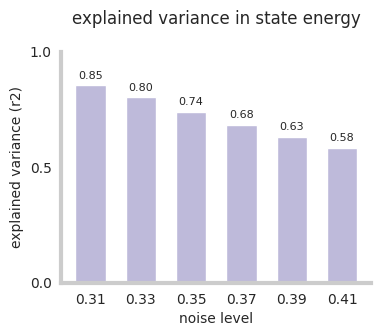
\includegraphics[width=0.7\linewidth]{files/expl_variance_energy-9d9ad5f5dcb888b9398d5cb2e1e6c7f2.png}
\caption[]{\textbf{Explained variance in state energy by first two principal components.} See \href{https://github.com/pni-lab/connattractor/blob/master/notebooks/supplemental\_material.ipynb}{supplemental\_material.ipynb} for details.}
\label{si_expl_variance_energy}
\end{figure}

\begin{figure}[!htbp]
\centering
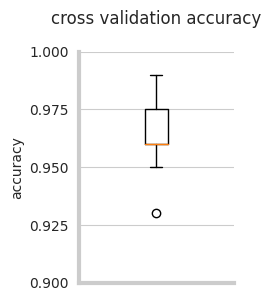
\includegraphics[width=0.7\linewidth]{files/classification_acc_s-c65939cd83b4f768e45adf14fd412309.png}
\caption[]{\textbf{Cross-validation classification accuracy of the fcHNN, when predicting the attractor state from state
activation.}  See \href{https://github.com/pni-lab/connattractor/blob/master/notebooks/supplemental\_material.ipynb}{supplemental\_material.ipynb} for details.}
\label{si_classification_acc_state_basins}
\end{figure}

\begin{figure}[!htbp]
\centering
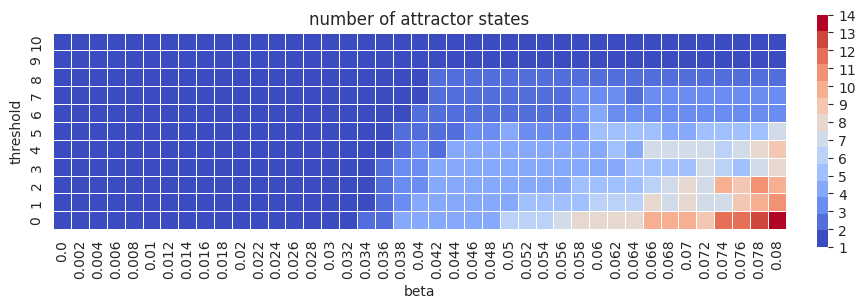
\includegraphics[width=0.7\linewidth]{files/att_state_emergence_-a406f7335bbdc27fb4bd9bec781fa95d.png}
\caption[]{\textbf{Parameter sweep of fcHNN parameters threshold and beta.} the number of attractor states is color-coded. See \href{https://github.com/pni-lab/connattractor/blob/master/notebooks/supplemental\_material.ipynb}{supplemental\_material.ipynb} for details.}
\label{si_att_state_emergence_over_beta}
\end{figure}

\begin{figure}[!htbp]
\centering
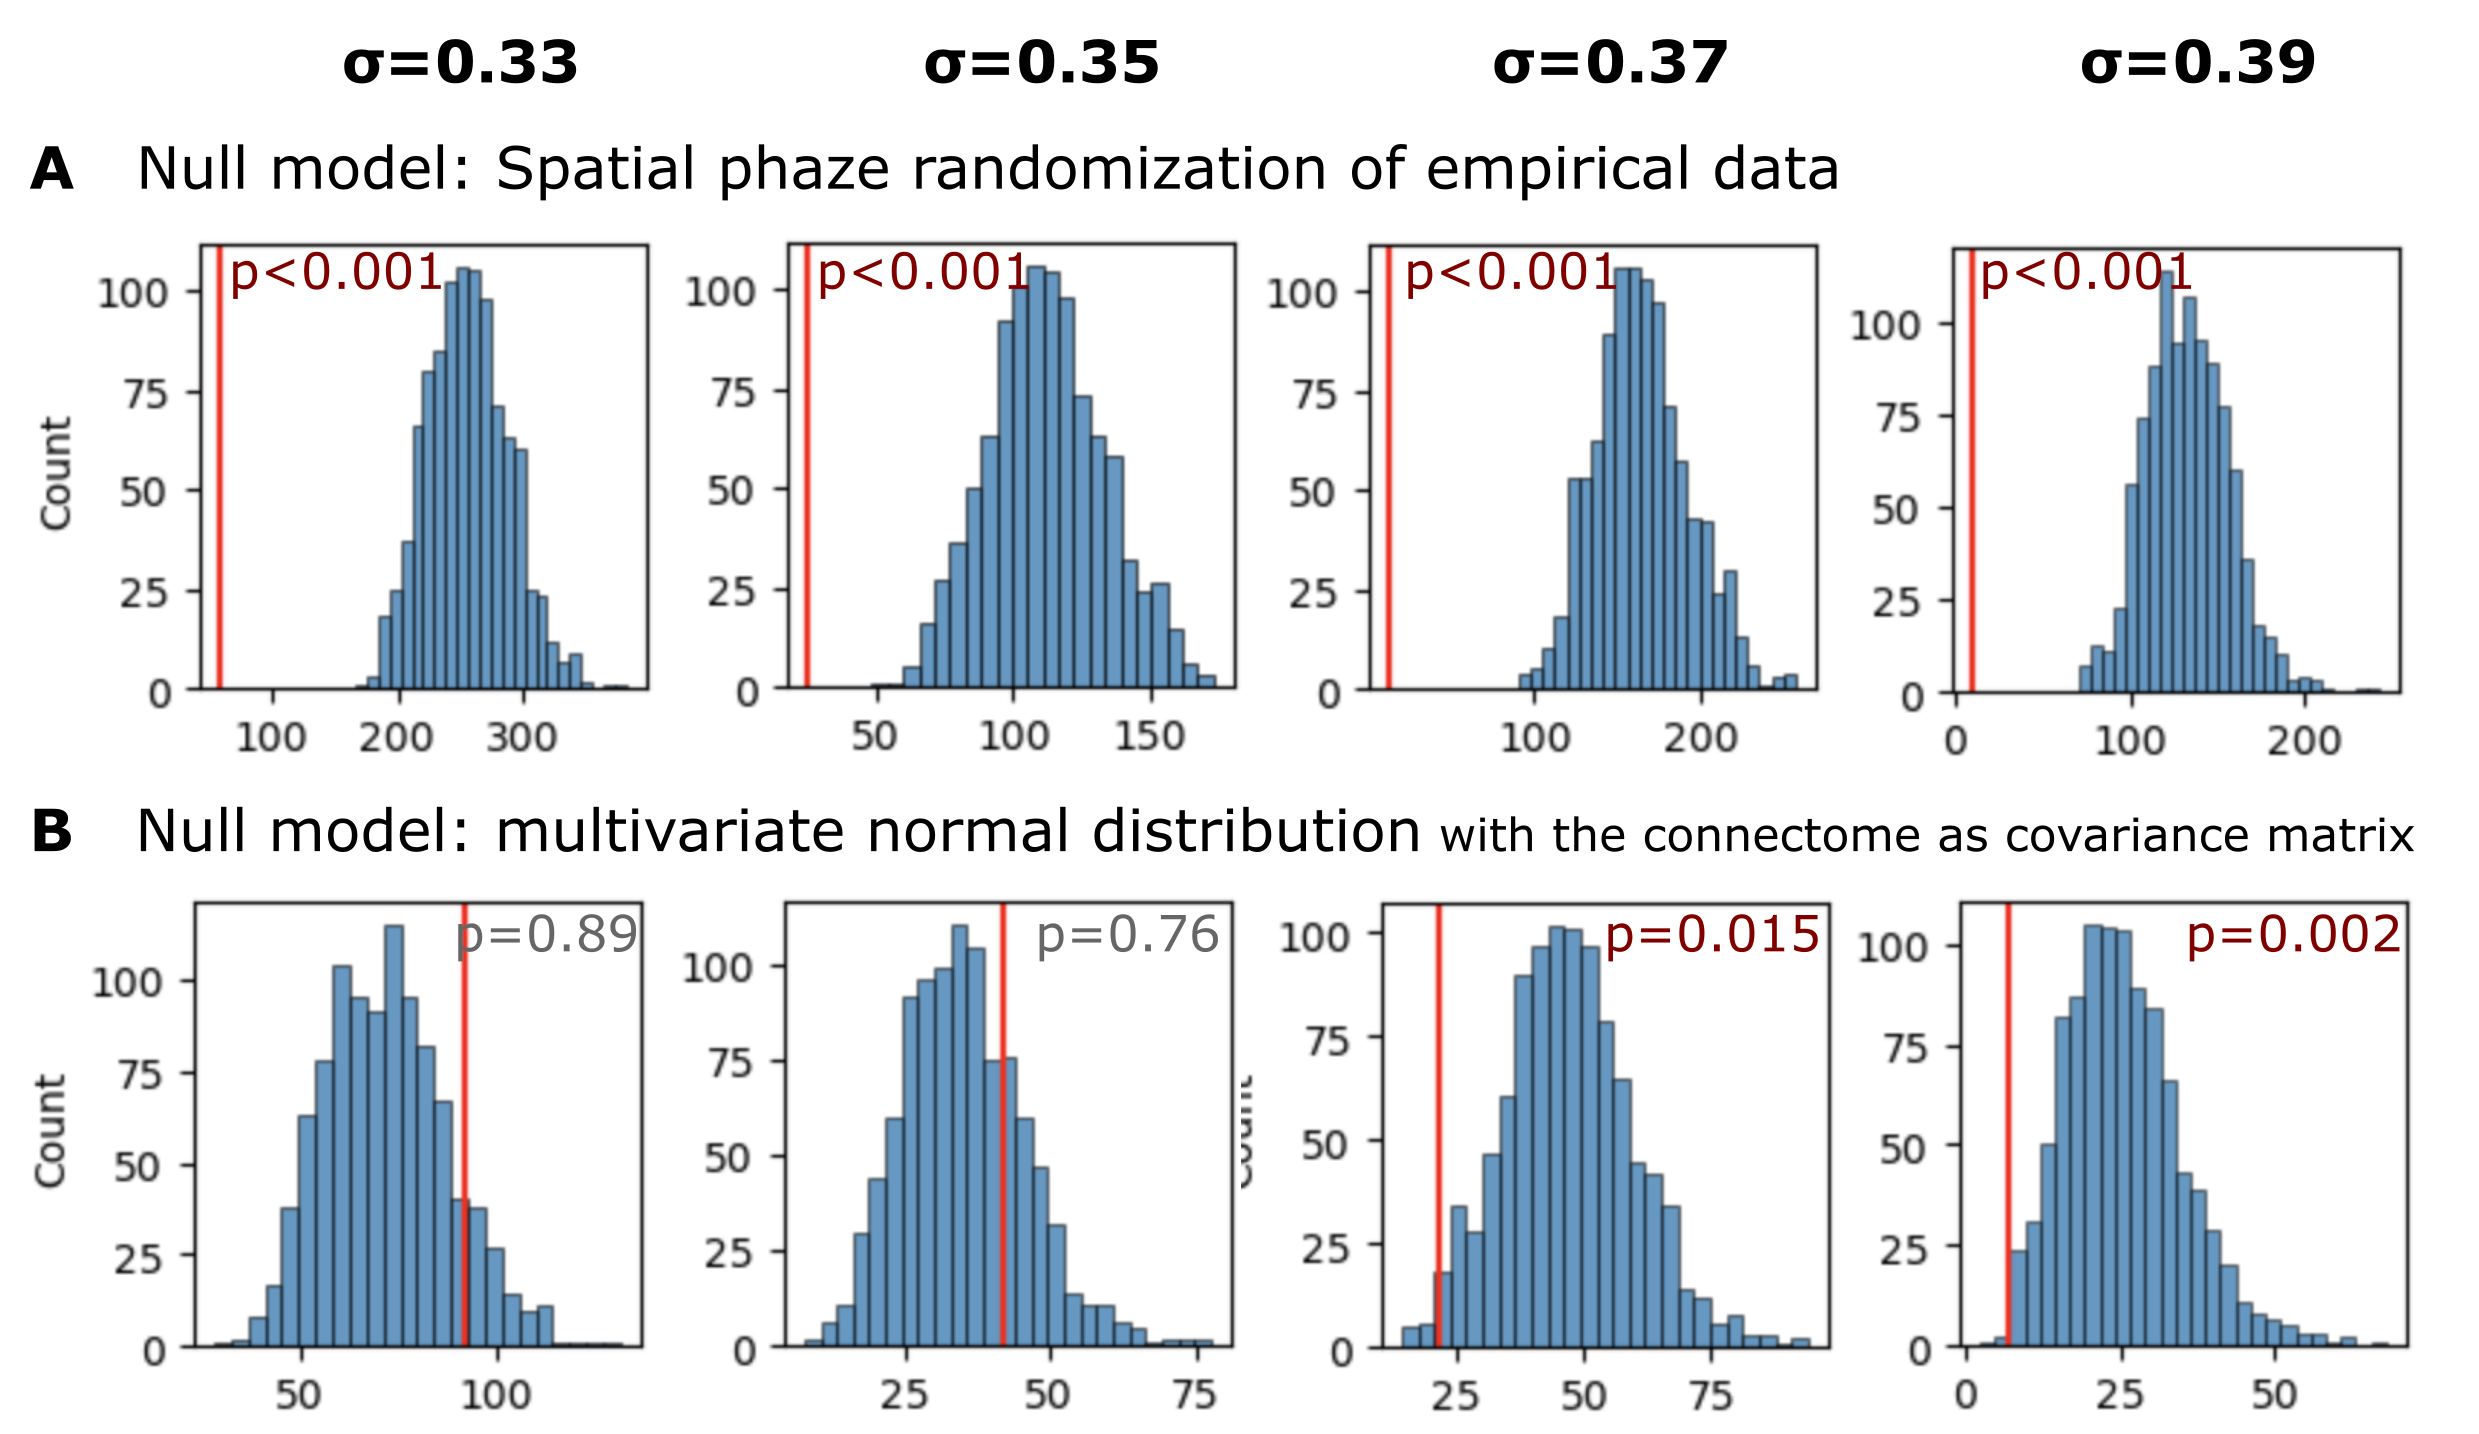
\includegraphics[width=0.7\linewidth]{files/si_state_occupancy_n-645b172c5a572f7b0a7efcc0648b53d1.png}
\caption[]{\textbf{Statistical inference of the fcHNN state occupancy prediction with different null models.}
\textbf{A} Results with a spatial autocorrelation-preserving null model for the empirical activity patterns. See \href{https://github.com/pni-lab/connattractor/blob/master/notebooks/null\_models.ipynb}{null\_models.ipynb} for more details.
\textbf{B} Results where simulated samples are randomly sampled from a multivariate normal distribution, with the functional connectome as the covariance matrix, and compared to the fcHNN performance. See \href{https://github.com/pni-lab/connattractor/blob/master/notebooks/supplemental\_material.ipynb}{supplemental\_material.ipynb} for details.}
\label{si_state_occupancy_null_models}
\end{figure}

\begin{figure}[!htbp]
\centering
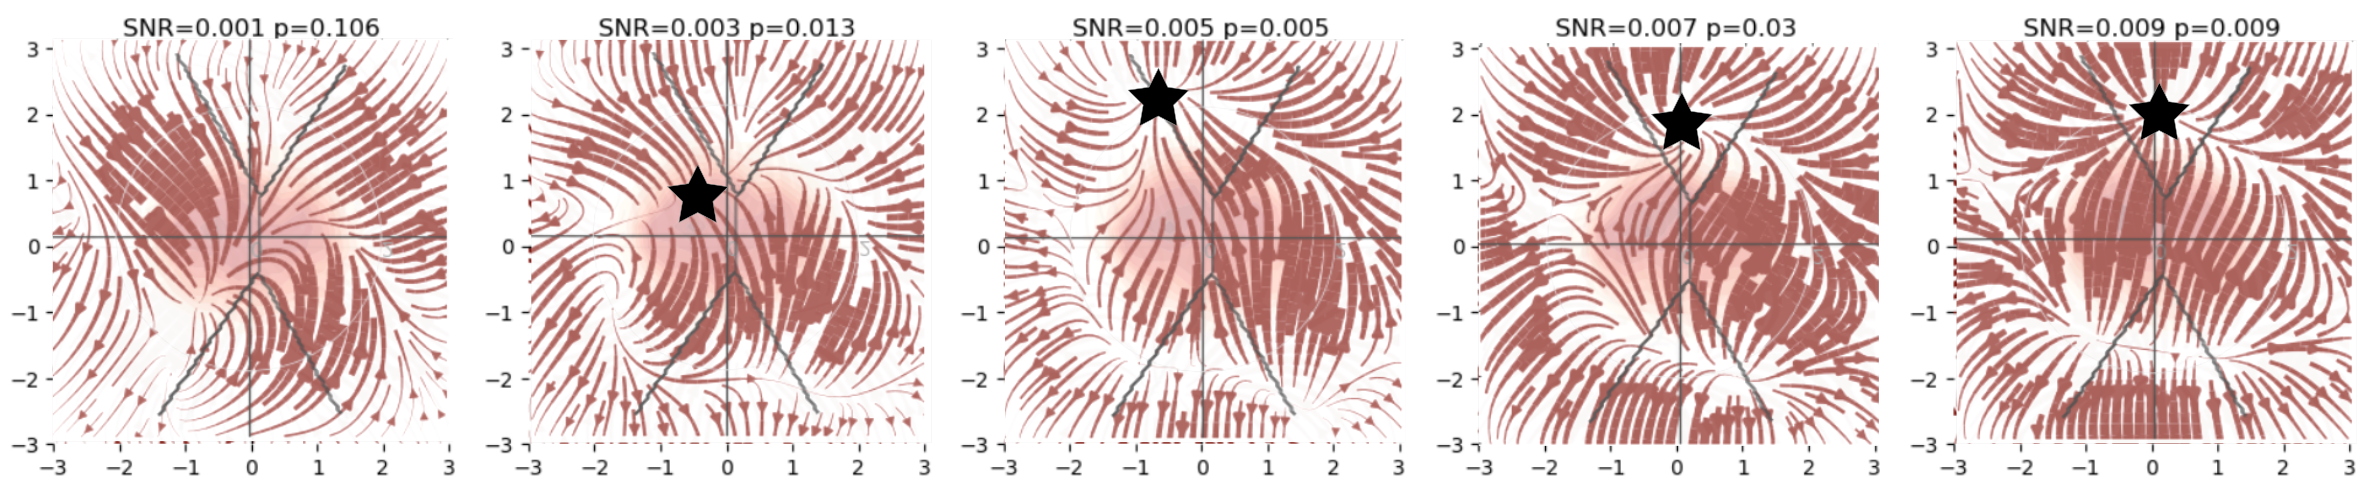
\includegraphics[width=0.7\linewidth]{files/si_pain_ghost_attrac-c0412d6aa9519aff8f20de1729f0c843.png}
\caption[]{\textbf{FcHNN can reconstruct the pain ``ghost attractor''.}
Signal-to-noise values range from 0.003 to 0.009. Asterisk denotes the location of the simulated ``ghost attractor''. P-values are based on permutation testing, by randomly changing the conditions in a per-participant basis. See \href{https://github.com/pni-lab/connattractor/blob/master/notebooks/main\_analyses.ipynb}{main\_analyses.ipynb} for more details.}
\label{si_pain_ghost_attractor_sim}
\end{figure}

\begin{figure}[!htbp]
\centering
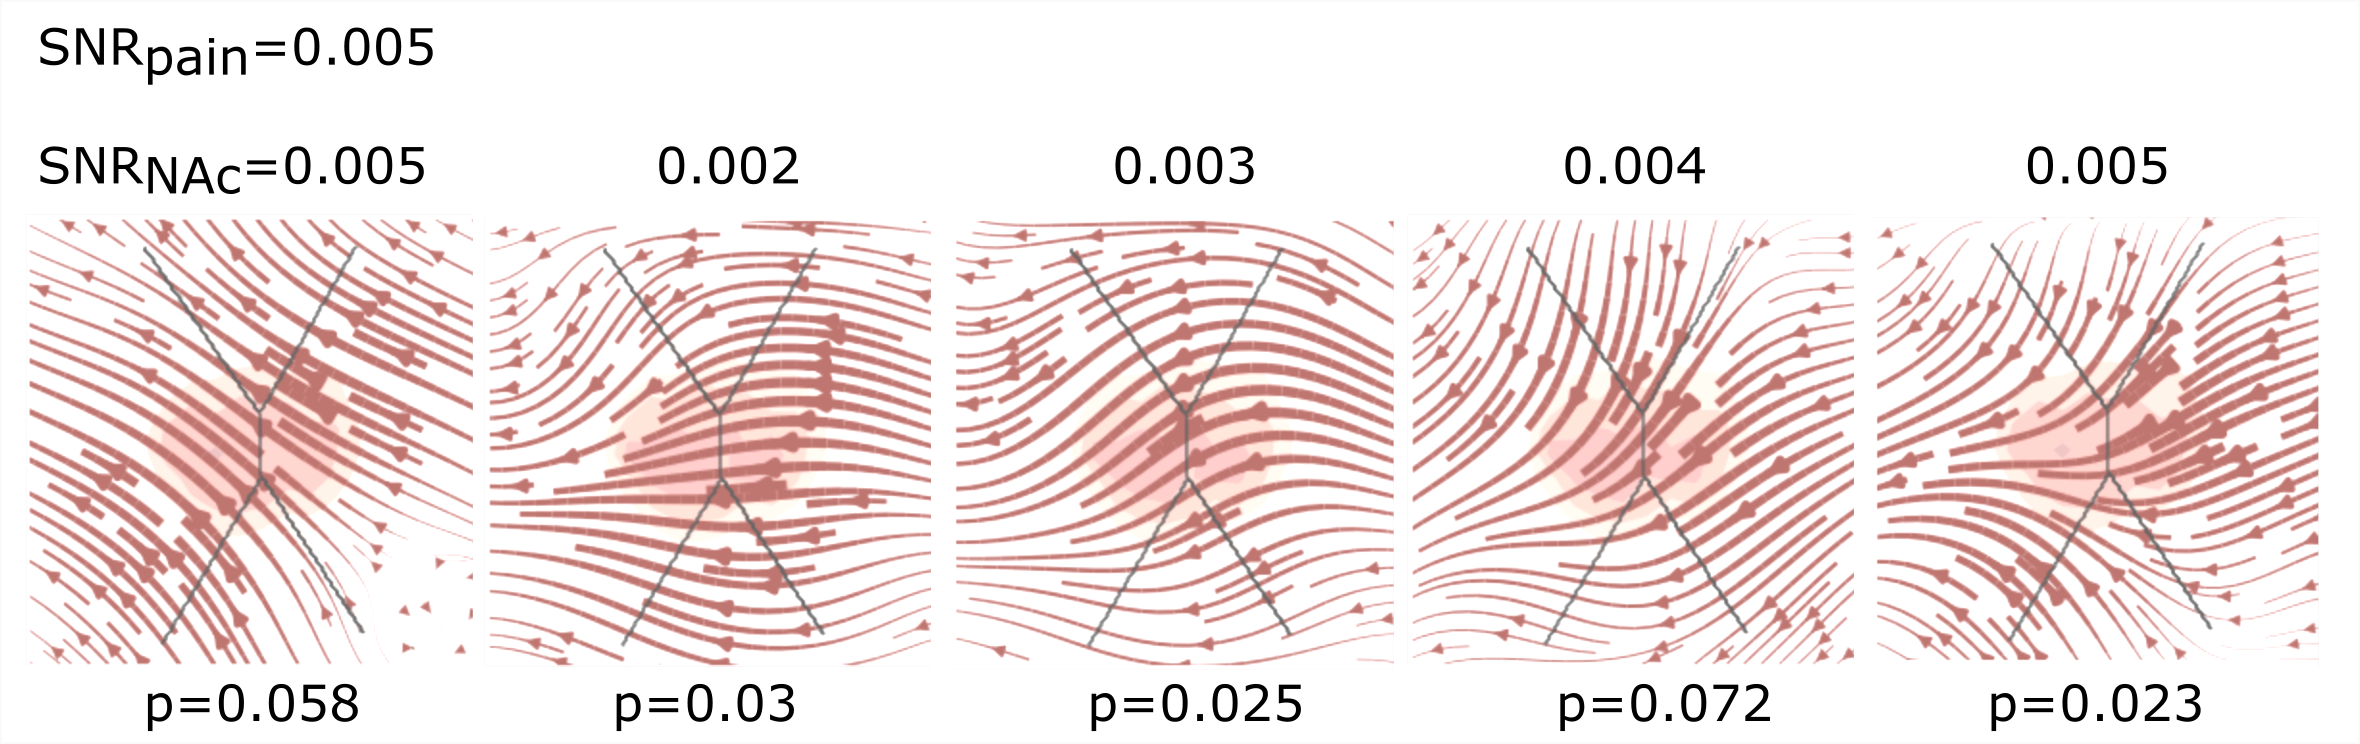
\includegraphics[width=0.7\linewidth]{files/si_downreg_trajector-682f780caa5f21f8c78daa47dd678da0.png}
\caption[]{\textbf{FcHNN can reconstruct the changes in brain dynamics caused by the voluntary donwregulation of pain (as contrasted to upregulation)}
Signal-to-noise values range from 0.001 to 0.005. P-values are based on permutation testing, by randomly changing the conditions in a per-participant basis. See \href{https://github.com/pni-lab/connattractor/blob/master/notebooks/main\_analyses.ipynb}{main\_analyses.ipynb} for more details.}
\label{si_downreg_trajectory_sim}
\end{figure}

\begin{figure}[!htbp]
\centering
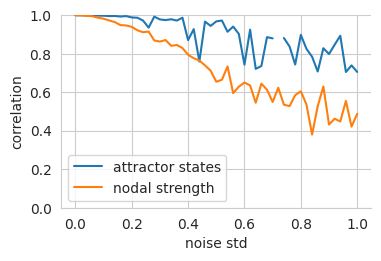
\includegraphics[width=0.7\linewidth]{files/noise_robustness_wei-0088e46f59fa81a72a26340f4eb8ffa2.png}
\caption[]{\textbf{Robustness of the fcHNN weights to noise.}
We set the temperature of the fcHNN, so that two attractor states emerge and iteratively add noise to the connectome.
To account for the change in dynamics, we adjust the temperature (beta) of the noisy fcHNN so that exactly two states emerge. We then highlight the decrease in nodal strength of the noisy connectome (the fcHNN weights) as a reference metric
vs the correlation of the attractor states that emerge from the noisy connectome. See \href{https://github.com/pni-lab/connattractor/blob/master/notebooks/supplemental\_material.ipynb}{supplemental\_material.ipynb} for details.}
\label{si_noise_robustness_weights}
\end{figure}

\begin{figure}[!htbp]
\centering
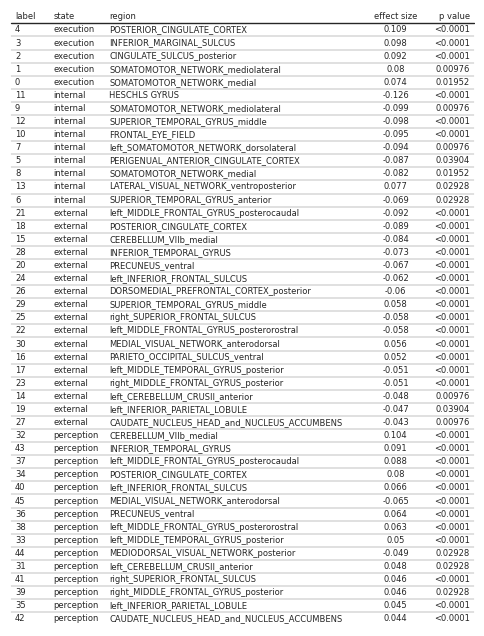
\includegraphics[width=0.7\linewidth]{files/clinical_results_tab-ab95084f242b0cff77efacf754a83d7e.png}
\caption[]{\textbf{All significant differences of the mean state activation analysis on the ABIDE dataset; label denotes the region
in the BASC122 atlas.} See \href{https://github.com/pni-lab/connattractor/blob/master/notebooks/supplemental\_material.ipynb}{supplemental\_material.ipynb} for details.}
\label{si_clinical_results_table}
\end{figure}

\subsection{Supplementary Tables}

\begin{table}
\centering
\caption[]{\textbf{Neurosynth meta-analyses.} The table includes details about the term used for the automated meta-analyses, as well as the number of studies included in the meta-analysis, the total number of reported activations and the maximal Z-statistic from the meta-analysis.}
\label{si-tab-neurosynth}
\begin{tabular}{p{\dimexpr 0.250\linewidth-2\tabcolsep}p{\dimexpr 0.250\linewidth-2\tabcolsep}p{\dimexpr 0.250\linewidth-2\tabcolsep}p{\dimexpr 0.250\linewidth-2\tabcolsep}}
\toprule
search term & num. studies & num. activations & max. Z \\
\hline
pain & 516 & 23295 & 14.8 \\
motor & 2565 & 109491 & 22.5 \\
auditory & 1252 & 46557 & 25.3 \\
visual & 3110 & 115726 & 15.4 \\
face & 896 & 31842 & 26.8 \\
autobiographical & 143 & 7251 & 15.7 \\
theory of mind & 181 & 7761 & 15.1 \\
sentences & 356 & 13461 & 16.5 \\
\bottomrule
\end{tabular}
\end{table}

\subsection{Supplementary Methods}

\textbf{Study 4 instructions for upregulation.}
\textit{``During this scan, we are going to ask you to try to imagine as hard as you can that the thermal stimulations are more painful than they are. Try to focus on how unpleasant the pain is, for instance, how strongly you would like to remove your arm from it. Pay attention to the burning, stinging and shooting sensations. You can use your mind to turn up the dial of the pain, much like turning up the volume dial on a stereo. As you feel the pain rise in intensity, imagine it rising faster and faster and going higher and higher. Picture your skin being held up against a glowing hot metal or fire. Think of how disturbing it is to be burned, and visualize your skin sizzling, melting and bubbling as a result of the intense heat.''}

\textbf{Study 4 instructions for downregulation.}
\textit{``During this scan, we are going to ask you to try to imagine as hard as you can that the thermal stimulations are less painful than they are. Focus on the part of the sensation that is pleasantly warm, like a blanket on a cold day. You can use your mind to turn down the dial of your pain sensation, much like turning down the volume dial on a stereo. As you feel the stimulation rise, let it numb your arm, so any pain you feel simply fades away. Imagine your skin is very cool, from being outside, and think of how good the stimulation feels as it warms you up.''}
%%%%%%%%%%%%%%%%%%%%%%%%%%%%%%%%%%%%%%%%%%%%%%%%%%
%%%%%%%%%%%%%%  acronyms & glossary  %%%%%%%%%%%%%
\printglossaries
%%%%%%%%%%%%%%%%%%%%%%%%%%%%%%%%%%%%%%%%%%%%%%%%%%




\bibliographystyle{unsrtnat}
\bibliography{main.bib}

\end{document}
